\chapter{Fundamentos Teóricos y Tecnológicos}
\label{chap:fundamentos}

\lettrine{E}{n} este capítulo, se expondrán los fundamentos teóricos y tecnológicos necesarios para comprender este trabajo. Además se comentarán las herramientas en las que nos apoyamos para llevar a cabo esta tarea.

\section{LiDAR}

El término LiDAR se proviene de “Light Detection and Ranging” en inglés. Esta tecnología utiliza un pulsoláser para medir con precisión las distancias y crear una representación tridimensionales de un entorno u objeto.

Su funcionamiento es el siguiente, en un emisor emite un pulso láser hacia una superficie u objeto, mientras que un receptor registra el tiempo que tarda en recibir los rebotes de ese pulso. Esto nos permite obtener con precisión la distancia entre el sensor y el objeto. En nuestro caso al trabajar con datos geoespaciales también es necesario que el sistema esté equipado con un GPS para obtener la ubicación geográfica del sensor.


\begin{figure}[h]
\centering
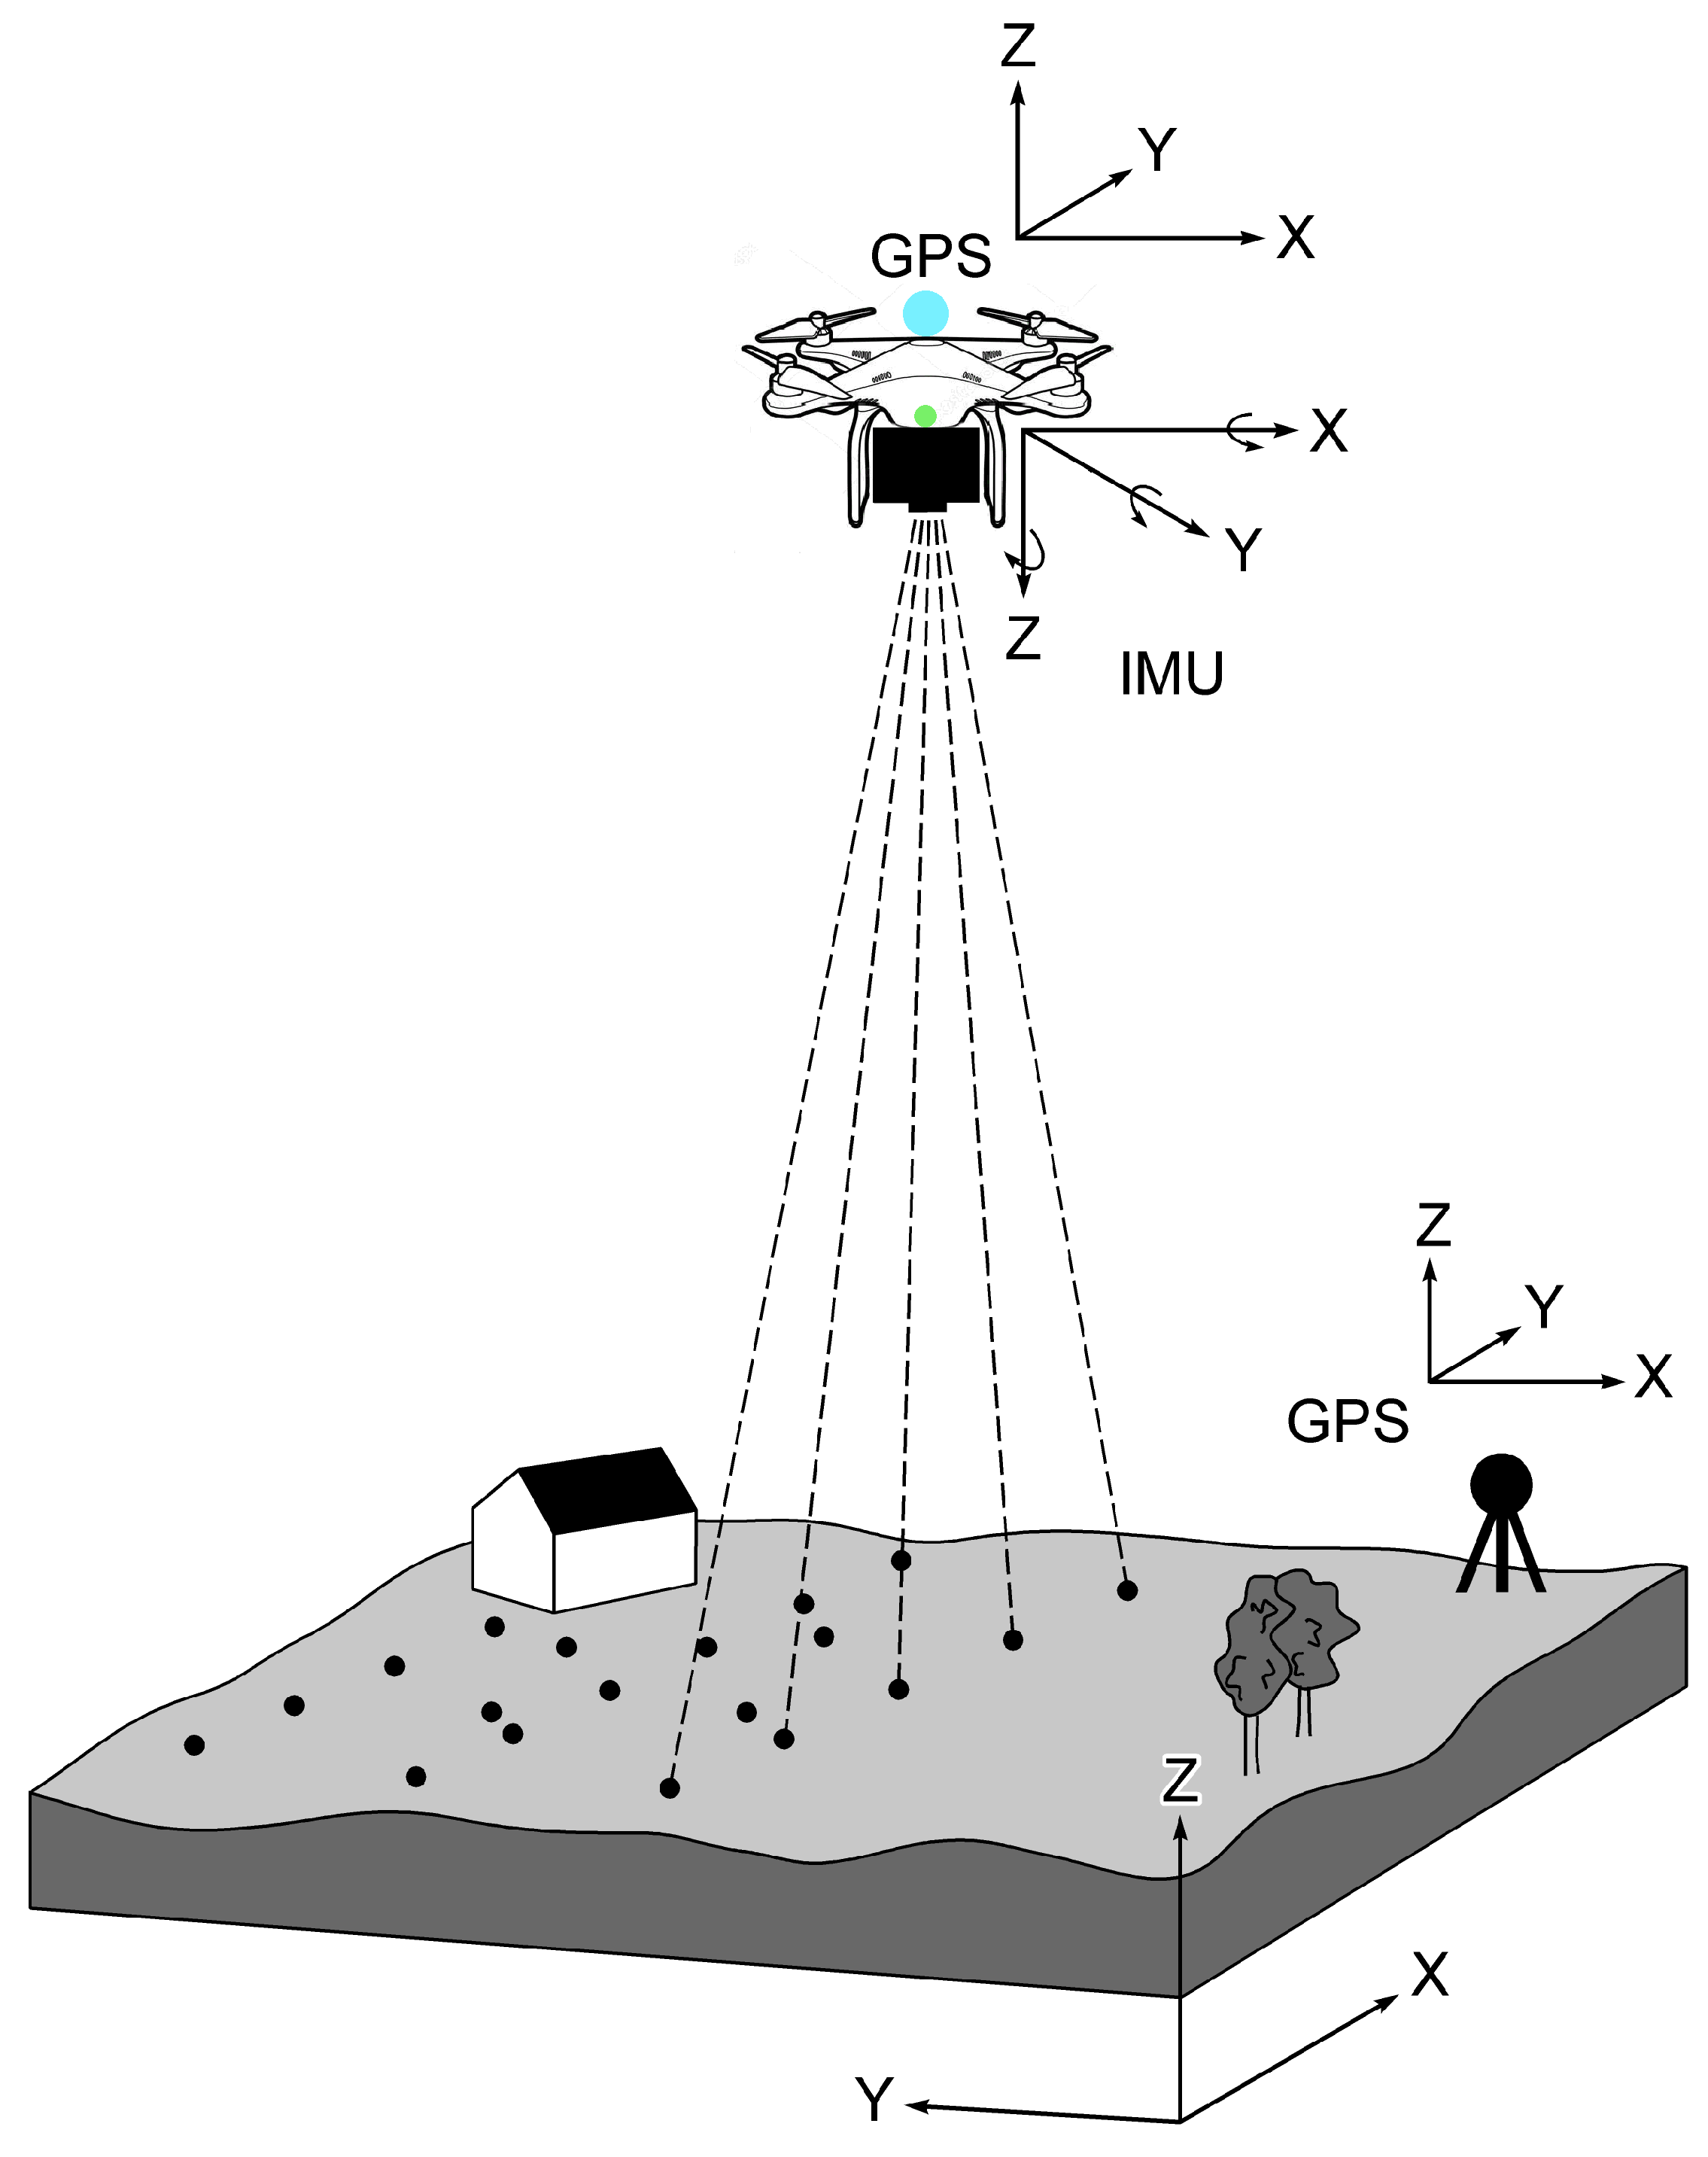
\includegraphics[width=6cm]{imaxes/remotesensing-10-01094-g001.png}
\label{fig:uavsensor}
\caption{Ejemplo de un sistema LiDAR en un UAV \cite{rs10071094}}
\end{figure}


En los últimos años esta tecnología ha experimentado un gran crecimiento debido a su versatilidad y capacidad para ser usado en multitud de escenarios. Entre estos estan el uso en vehículos de conducción autónoma \cite{articleauto}, gestión forestal, como este trabajo, \cite{rs14010170}, para arqueología \cite{lidararque}, agricultura de precision \cite{RIVERA2023107737} o para obtener modelos 3d de ciudades \cite{lidarcity}.

\subsection{Nubes de Puntos}
Las nubes de puntos son el resultado del escaneo de una superficie u objeto, esta nube de puntos no es mas que un conjunto de puntos tridimensionales. Cada uno de estos puntos guarda su coordenada (x, y, z).El par de coordenadas (x, y) representan la ubicación en el plano, y la coordenada (z) la altura de ese punto. Junto con esto también se guardan atributos adicionales para tener mas información de los objetos y superficies. A continuación, explicaremos los más importantes para nuestro trabajo.


\subsubsection{Numero de Retornos}
Existen escenarios en los que un mismo pulso láser puede impactar en superficies con múltiples capas, como ocurre en el caso de un edificio o un árbol. Cada vez que un rayo regresa al sensor, lo denominamos "retorno".

Un símil que puede ayudarnos a comprender mejor esto sería pensar en cuando lanzamos una pelota contra una pared y esta rebota varias veces antes de ser recogida. Cada rebote representaría un "retorno" de la pelota.

En nuestra nube de puntos, registramos cada uno de estos "rebotes" como puntos individuales. Esta información resulta útil para comprender objetos con múltiples capas, como los árboles, que son el objeto de estudio en este trabajo. Específicamente, como veremos más adelante, utilizaremos el primer retorno, ya que en la mayoría de los casos representa la parte superior del árbol, conocida como "corona arbórea".

\subsubsection{Clasificación del objeto}
Cada punto en la nube de puntos puede ser clasificado según su origen. Por ejemplo, si los puntos pertenecen al suelo, edificios o vegetación. Para que esta clasificación sea consistente y homogénea entre todas las nubes de puntos la Sociedad Americana de Fotogrametría y Sensores Remotos (ASPRS) \cite{ASPRS-LAS} propone los siguiente códigos a la hora de clasificar los puntos \ref{tabclas}.

\begin{table}[hp!]
   \centering
  \rowcolors{2}{white}{udcgray!25}
  \begin{tabular}{c|c}
  \rowcolor{udcpink!25}
  \textbf{Valor de clasificación} & \textbf{Significado} \\\hline
  
  0 & Nunca clasificado \\
  1 & No asignado \\
  2 & Terreno  \\
  3 & Vegetación baja  \\
  4 & Vegetación media \\
  5 & Vegetación alta  \\
  6 & Edificio \\
  7 & Punto bajo \\
  8 & Reservado \\
  9 & Agua  \\
  10 & Ferrocarril   \\
  11 & Superficie de la carretera   \\
  12 & Reservado   \\
  13 & Protector de cable (señal)   \\
  14 & Conductor de cable (fase)   \\
  15 & Torre de transmisión   \\
  16 & Conector de la estructura de cables (aislante)   \\
  17 & Plataforma del puente \\
  18 & Ruido alto \\
  19-63 & Reservado \\
  64-255 & Definido por el usuario 

  \end{tabular}

  \caption{Códigos de clasificación LAS definidos por ASPRS para las versiones LAS 1.1 a 1.4}
  \label{tabclas}


\end{table}

\subsubsection{Densidad de puntos}
Este valor representa la cantidad de puntos en una región específica, lo que puede proporcionar detalles sobre la complejidad del objeto o la resolución del escaneo. Para este proyecto, es importante tener regiones con altas densidades de puntos para ser capaces de reconocer la estructura del árbol, tanto la copa como el tronco.

\vspace{0.5cm}

Una vez comprendido qué conforma una nube de puntos, necesitamos entender cómo se guardan estos datos. El formato más ampliamente utilizado es el LAS (LiDAR Data Exchange Format), desarrollado por la ya mencionada Sociedad Americana de Fotogrametría y Sensores Remotos. Este formato es altamente eficiente y permite diferentes niveles de compresión. Al ser el formato más extendido, será el más utilizado por las herramientas de procesamiento y visualización.

Como alternativa a este formato, y también muy utilizado, tenemos el LAZ, un formato que utiliza técnicas de compresión sin pérdida para reducir el tamaño del archivo sin perder precisión. Normalmente, los datos LAS se pueden convertir a LAZ sin ningún problema y posteriormente, para su procesamiento, se pueden volver a descomprimir.

\section{Detección de Objetos}

La detección de objetos en nubes de puntos es una tarea crucial en diversas aplicaciones como la conducción autónoma, la planificación urbana o la robótica. Existen varias aproximaciones para realizar esto, cada una de con sus ventajas y limitaciones. Ahora expondremos algunas de las técnicas más comunes usadas en este ámbito:

\subsection{Segmentación basada en Clústeres}

La segmentación basada en clústeres agrupa puntos que están cerca unos de otros en clústeres, lo que permite identificar regiones que probablemente representen objetos o partes del entorno. Métodos como el crecimiento de regiones, K-means, Mean Shift y DBSCAN son ampliamente utilizados para esta técnica. La segmentación basada en clústeres es efectiva para detectar objetos con formas y tamaños variados.

\begin{figure}[h]
\centering
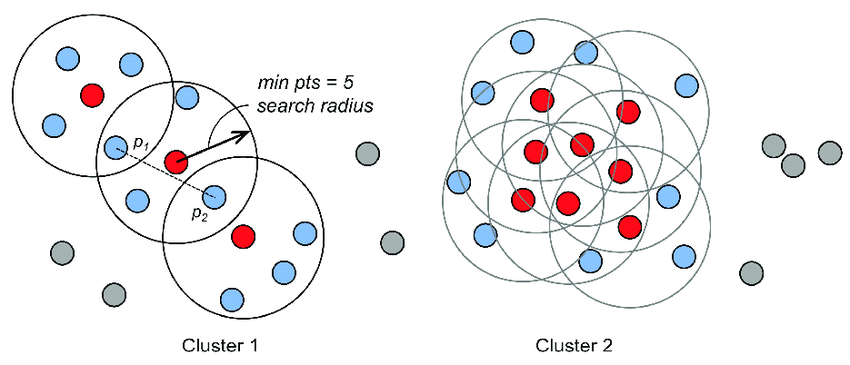
\includegraphics[width=10cm]{imaxes/The-DBSCAN-algorithm-and-two-generated-clusters-There-are-three-types-of-points-as.png}
\label{fig:pointnetc}
\caption{Ejemplo del funcionamiento del algoritmo de clustering \textit{dbscan} \cite{dbscan}}
\end{figure}


\subsection{Extracción de Características}

La extracción de características implica la identificación de atributos significativos de los puntos en una nube, como la altura, la intensidad del retorno, la densidad de puntos y la distribución espacial. Estos atributos se utilizan para identificar regiones que podrían contener objetos. Esta técnica es muy versátil y puede combinarse con otras para mejorar los resultados.


\subsection{Aprendizaje Automático (Machine Learning)}

El aprendizaje automático, como el uso de redes neuronales convolucionales (CNN) y métodos de aprendizaje profundo, permite a los sistemas aprender patrones complejos directamente de los datos. Los modelos se entrenan con datos etiquetados y luego se utilizan para detectar objetos en nuevas nubes de puntos. Esta técnica es eficaz para capturar relaciones no lineales y características sutiles.

\begin{figure}[h]
\centering
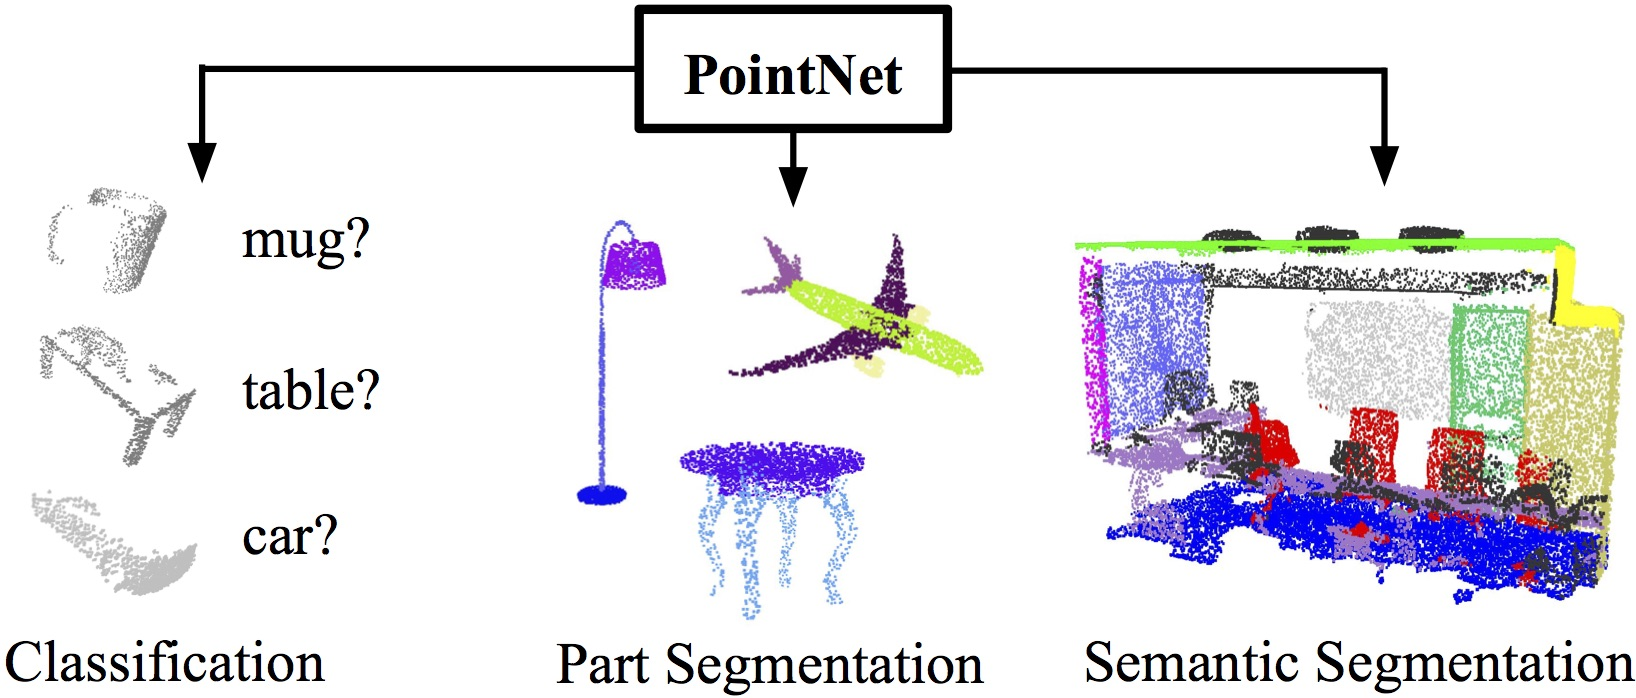
\includegraphics[width=10cm]{imaxes/teaser.jpg}
\label{fig:pointnetc}
\caption{Ejemplo de la red PointNet \cite{pointnet}}
\end{figure}


\subsection{Filtros Geométricos}
Los filtros geométricos son técnicas que eliminan puntos que no pertenecen a objetos sólidos, como el suelo o elementos del entorno. Filtros como el de plano y el de distancia se emplean para mantener solo los puntos relevantes para la detección de objetos.


\subsection{Análisis de Vecinos Cercanos}

El análisis de vecinos cercanos implica evaluar la distribución y proximidad de los puntos en la nube. Los puntos con suficientes vecinos cercanos en un área se consideran parte de un objeto o una superficie. Esta técnica es efectiva para detectar regiones densas y agrupaciones de puntos.


\section{Herramientas}
Para el procesado de nubes de puntos es necesario utilizar herramientas para visualizar y tratar los datos. En la mayoría de los lenguajes de programación tenemos disponibles bibliotecas o librerías que nos lo permiten, como por ejemplo, PDAL, de la cual hablaremos más adelante.
A continuación se presentaran las herramientas empleadas durante el desarrollo del trabajo.

\subsection{QT Reader}
Esta es una herramienta gráfica muy sencilla que nos permite visualizar nubes de puntos con una interfaz simple, concisa y veloz. Esta herramienta nos permite utilizar los formatos más comunes, como LAS o LAZ.

\begin{figure}[h]
\centering
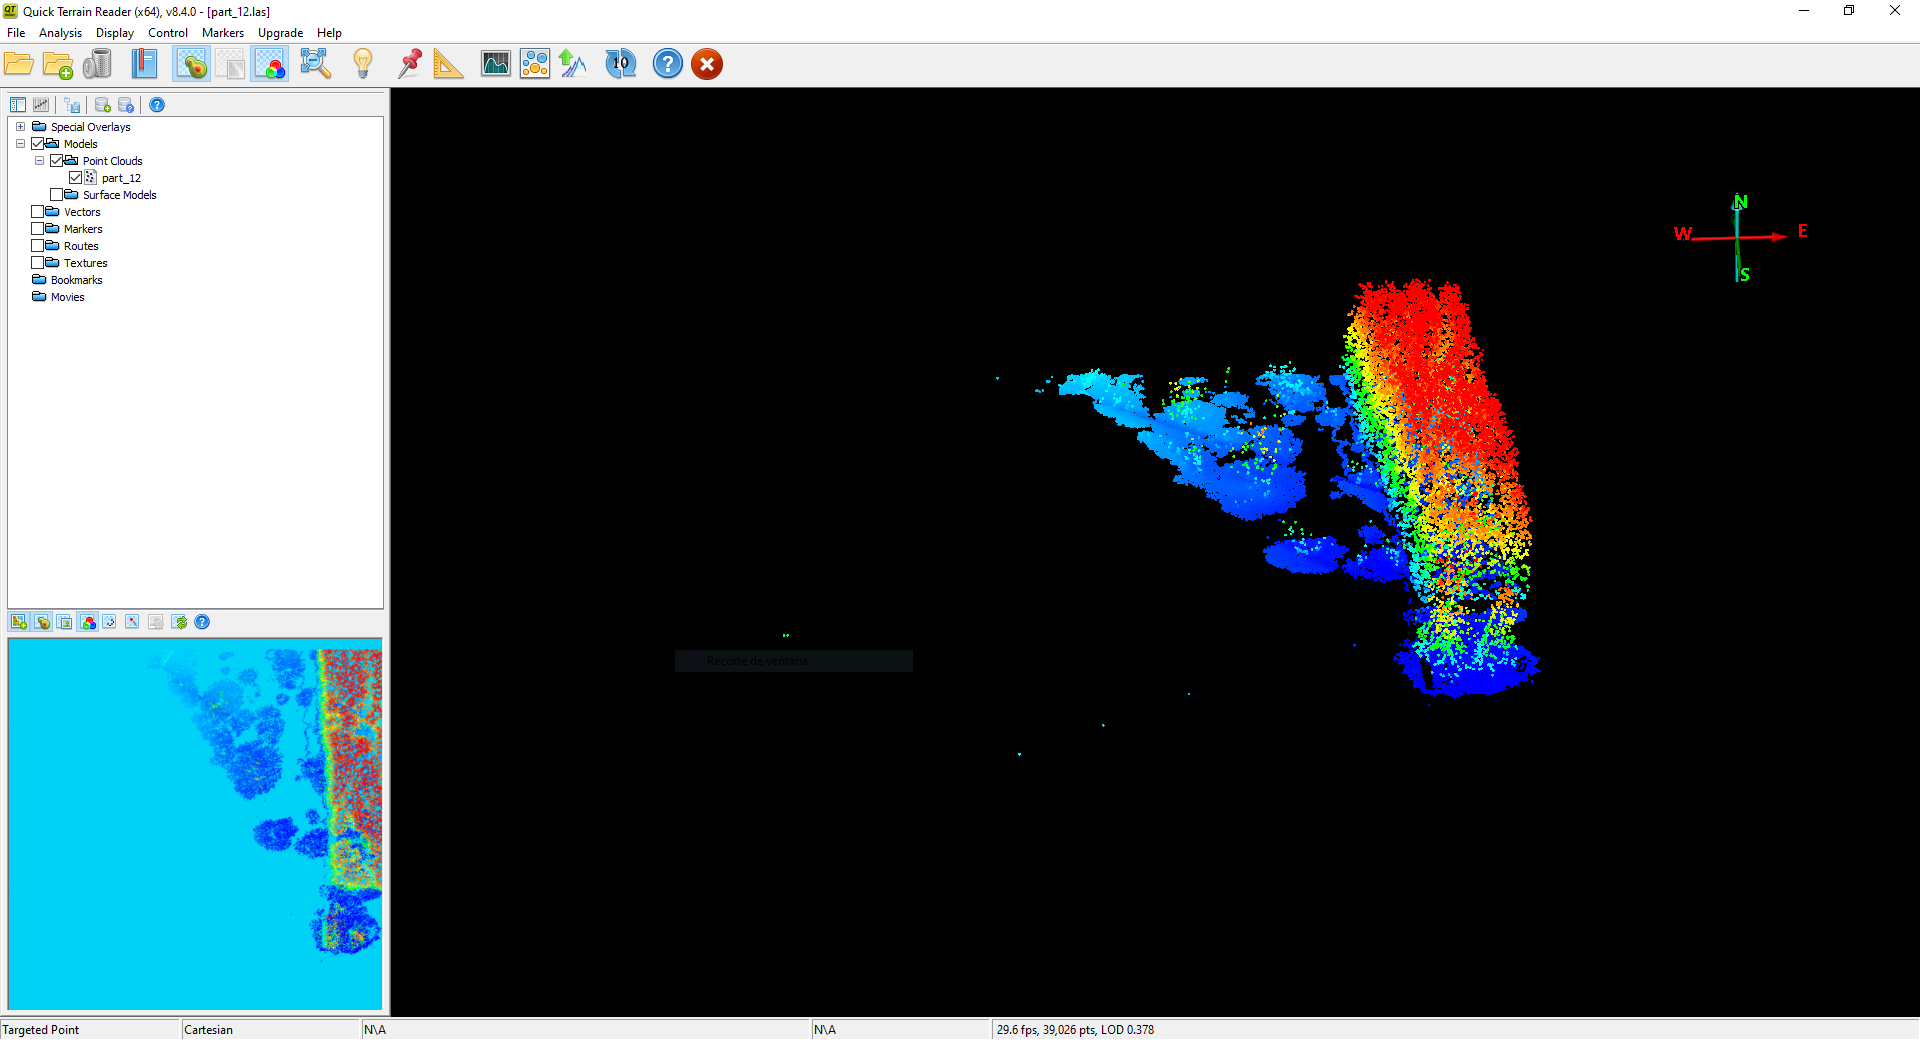
\includegraphics[width=10cm]{imaxes/qtreaderventana.png}
\label{fig:pointnetc}
\caption{Interfaz de QR Reader}
\end{figure}

\subsection{PADL}

PDAL (Point Data Abstraction Library) es una biblioteca de código abierto desarrollada en C++ para procesar y analizar datos de nubes de puntos en 3D. Nos permite leer, escribir, filtrar y transformar datos en los principales formatos. Además, cuenta con bibliotecas que permiten su utilización en varios lenguajes diferentes \cite{pdal}.

\subsection{Open3D}
Es otra biblioteca de código abierto para el procesamiento y visualización de nubes de puntos. En este proyecto, se utilizó debido a las herramientas que ofrece para la visualización interactiva de las nubes de puntos \cite{Open3d}.

\subsection{WhiteBox Tools}
Esta es una herramienta para el procesamiento de nubes de puntos que consta de diversos algoritmos diseñados para el procesamiento de datos LiDAR \cite{Whitebox}.

\subsection{Python}
Es un lenguaje de alto nivel muy flexible, con una amplia variedad de bibliotecas disponibles tanto para el procesamiento de datos LiDAR como para matemáticas. Este es el lenguaje sobre el cual se basa toda nuestra implementación \cite{python}.

\subsection{Conda}
Es un gestor de paquetes y un sistema de administración de entornos para lenguajes como Python. Permite instalar y gestionar paquetes; en nuestro caso, se usó para hacer uso de PDAL \cite{conda}.


